\setcounter{section}{1}

\Needspace{5\baselineskip}
\hypertarget{ux6a21ux578bux4e0aux4e0bux6587ux534fux8bae}{%
\section{模型上下文协议}\label{ux6a21ux578bux4e0aux4e0bux6587ux534fux8bae}}

模型上下文协议（Model Context Protocol，简称MCP）是由Anthropic于2024年11月推出的一项开源标准协议。它是模型侧和工具侧之间的协议，核心目标是为大型语言模型（LLM）提供一个标准化的接口，使其与外部数据源、工具和开发环境的接口匹配，主要在AI调用外部工具或读取外部工具时使用（如果工具代码或数据库读取代码已经全部封装在模型侧，就不需要）。

如果打个比方，MCP就像是AI界的``USB-C接口''。正如USB-C统一了各种电子设备的物理连接方式一样，MCP统一了AI应用与外部世界（如本地文件系统、企业数据库、API 服务等）的连接和交互标准。

\Needspace{5\baselineskip}
\hypertarget{ux4e00ux4ea7ux751fux80ccux666f-1}{%
\subsection{一、产生背景}\label{ux4e00ux4ea7ux751fux80ccux666f-1}}

大模型走向Agent，一个重要的问题是许多外部工具或私有数据是由对应领域的企业封装的，需要让模型厂商的模型侧接口和外部企业提供的接口匹配，才能调用这些工具，而不同的模型厂商（如 OpenAI、Anthropic、Google）有各自实现工具调用的数据结构。开发者如果想让一个内部的数据库查询工具同时支持GPT和Claude，必须编写和维护多套适配层代码。

MCP 通过定义一套独立于模型厂商的通用协议，实现了``一次开发，多模运行''。工具开发者只需按照MCP标准封装一次系统能力，即可被任何支持该协议的AI客户端统一调度。

\Needspace{5\baselineskip}
\hypertarget{ux4e8cux6838ux5fc3ux67b6ux6784}{%
\subsection{二、核心架构}\label{ux4e8cux6838ux5fc3ux67b6ux6784}}

\begin{figure}[htbp]
\centering
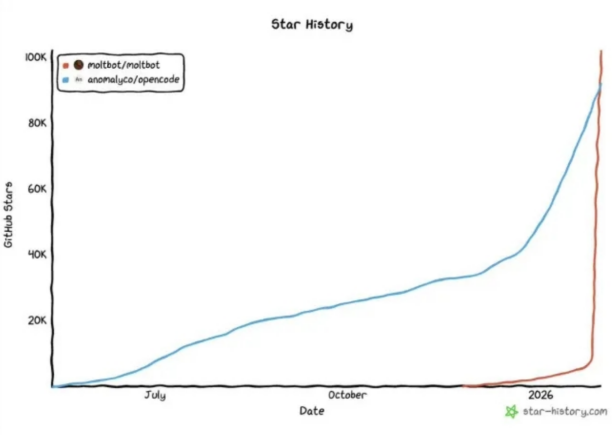
\includegraphics{images/image-0035.png}
\caption{MCP Host、Client 与 Server 的交互架构}
\end{figure}

MCP Host：用户直接交互的AI应用程序或环境，例如Claude Desktop、Cursor等，在模型侧，内部运行着LLM。LLM需要调用工具时，Host根据LLM输出的调用工具名称，找到对应的MCP Client。

MCP Client（客户端）：嵌入在模型侧的Host内部，是LLM与外部资源之间的``翻译官''。一个Host可以管理多个逻辑Client或连接器，由它们与对应的Server通信。Client负责构造符合MCP标准的结构化请求，并处理能力发现、工具调用路由、返回结果和错误信息。在MCP 2026-07-28版本中，核心协议已经改为无状态请求，不能再假定Client必须维护旧版协议中的持久会话。

MCP Server（服务器）：轻量级的独立程序，在外部工具或数据侧。每一个服务器都对应着一项或多项具体的能力，包括工具（可以执行的动作或函数）和资源（只读）。它可以是本地脚本，也可以是云端服务。Server向Client暴露自身的工具和数据读取能力，并在接收到标准指令后执行相应操作，将格式化后的结果返回给Client。

\Needspace{5\baselineskip}
\hypertarget{ux4e09ux5de5ux4f5cux6d41ux7a0b}{%
\subsection{三、工作流程}\label{ux4e09ux5de5ux4f5cux6d41ux7a0b}}

\begin{enumerate}
\def\labelenumi{\arabic{enumi}.}
\item
  协议版本与可选能力发现：在MCP 2026-07-28版本中，每个请求都会携带协议版本、客户端身份和能力信息，不再要求旧版的\texttt{initialize}/\texttt{initialized}握手或\texttt{Mcp-Session-Id}。如果Client希望在调用工具前了解Server支持的版本和能力，可以先调用可选的\texttt{server/discover}；也可以直接发送具体请求并处理不支持的版本或方法错误。
\item
  能力列表获取：Client可以通过\texttt{tools/list}、\texttt{resources/list}等方法获取Server当前公开的Tools和Resources，包括工具名称、用途和参数Schema。Host再根据自身的上下文管理策略，把必要的工具描述提供给LLM。为了保证工具的可扩展性、避免上下文爆炸并尽量保证缓存命中，也可以只暴露工具目录或``元工具''，再按需加载具体工具定义。
\item
  用户发起请求：用户向Host提出问题，例如：``帮我查一下昨天数据库里新增了多少付费用户，并生成一份总结''。
\item
  LLM决策与指令生成：Host将用户的问题连同Server提供的工具列表一并发送给大模型进行推理。LLM分析后判断需要使用``数据库查询''工具，于是生成符合Schema要求的工具调用指令。
\item
  路由与执行：Host根据指令，将其路由到内部对应的Client。Client把工具调用封装为MCP的JSON-RPC请求，并在请求中携带当前协议版本等必要元数据，再发送给对应的Server。Server执行SQL查询并获取数据，然后将结果返回给模型侧的Client。
\item
  上下文回传与最终响应：Client将查询结果作为新的上下文信息补充给大模型。LLM基于这些真实取回的数据进行逻辑推理，生成自然语言回答，最终由Host展示给用户。
\end{enumerate}

\FloatBarrier
\Needspace{5\baselineskip}
\hypertarget{ux53c2ux8003ux6587ux732e-123}{%
\subsection{参考文献}\label{ux53c2ux8003ux6587ux732e-123}}

\vspace{0.25em}
\begin{itemize}
\tightlist
\item
  Anthropic. (2024). \href{https://www.anthropic.com/news/model-context-protocol}{Introducing the Model Context Protocol}.
\item
  Soria Parra, D., \& Delimarsky, D. (2026). \href{https://blog.modelcontextprotocol.io/posts/2026-07-28/}{The 2026-07-28 Specification}. Model Context Protocol Blog.
\item
  Model Context Protocol. (2026). \href{https://modelcontextprotocol.io/specification/2026-07-28}{Specification (Protocol Revision 2026-07-28)}.
\end{itemize}

\clearpage
